% catalogue: title = Code as emitted by tikzfigure itself
% catalogue: min-coverage = 1.00
\documentclass[border=10pt]{standalone}
\PassOptionsToPackage{dvipsnames,svgnames,x11names}{xcolor}
\usepackage{tikz}
\usepackage{pgfplots}
\pgfplotsset{compat=newest}
\usepgfplotslibrary{groupplots}
\usetikzlibrary{arrows.meta}
\begin{document}
% --------------------------------------------- %
% Tikzfigure generated by tikzfigure v0.3.1     %
% https://github.com/max-models/tikzfigure      %
% --------------------------------------------- %
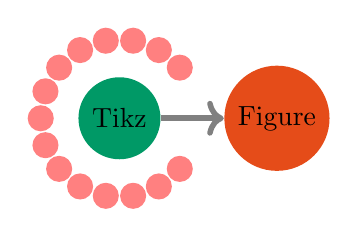
\begin{tikzpicture}
    \pgfmathsetmacro{\R}{1.0}
    % Define the layers library
    \pgfdeclarelayer{0}
    \pgfdeclarelayer{1}
    \pgfsetlayers{0,1}

    % Layer 0
    \begin{pgfonlayer}{0}
        \node[shape=circle, fill=blue!40!green] (node0) at ({0}, {0}) {Tikz};
        \node[shape=circle, fill=purple!40!orange] (node1) at ({2}, {0}) {Figure};
        \foreach \angle in {40,60,80,100,120,140,160,180,200,220,240,260,280,300,320}{
            \node[shape=circle, fill=red!50] () at ({\R*cos(\angle)}, {\R*sin(\angle)}) {};
        }
    \end{pgfonlayer}{0}

    % Layer 1
    \begin{pgfonlayer}{1}
        \draw[color=gray, line width=2, arrows=->] (node0) to (node1);
    \end{pgfonlayer}{1}
\end{tikzpicture}
\end{document}
